\documentclass{ximera}

\pgfplotsset{compat=1.6}

% MATH -----------------------------------------------------------
\newcommand{\nats}{\mathbb N}
\newcommand{\ints}{\mathbb Z}
\newcommand{\rats}{\mathbb Q}
\newcommand{\reals}{\mathbb R}
\newcommand{\complex}{\mathbb C}
\newcommand{\powerset}{\mathscr P}

%-------------------------------------------------------------


\begin{document}
\begin{abstract}
 \end{abstract}

    \title{Euler's Method}
    \maketitle

 Sometimes it is just not possible to solve an 1st order IVP $y'=f(x,y)$, $y(x_{0})=y_{0}$ analytically for an implicit or explicit solution.\\

 But you can estimate future values of the solution.  The following method is one way to do this,  called \textbf{Euler's method} (also called the $``$forward Euler" method):\\


 Suppose we are interested in finding the values of the solution $y$ at equally spaced values $x_{i}=x_{0}+i\Delta x$ for $i=1,2,...,n$ where $\Delta x$ is the $``$step size." \\

Denote by $y_{i}$ the approximate value $y(x_{i})$ (for $i=1,2,..,n$).  Then the \underline{absolute error at the ith step} is $e_{i}=|y(x_{i})-y_{i}|$ (for $i=1,2,..,n$). \\


 Euler's method rests on having the tangent line to the graph of the solution curve at $x_{i}$ approximate the curve on $[x_{i},x_{i+1}]$.  The slope at $(x_{i},y_{i})$ is $f(x_{i},y_{i})$  so the tangent line on $[x_{i},x_{i+1}]$ is  $$y=y_{i}+f(x_{i},y_{i})(x-x_{i}).$$

\vspace{1cm}

 So for $i=0$, we get the approximate value \\$y(x_1)\approx y_{1}=y_{0}+f(x_{0},y_{0})(x_{1}-x_{0})=y_{0}+ f(x_{0},y_{0})\Delta x$.\\


 Then we can repeat to get the approximate value \\$y(x_2)\approx y_{2}=y_{1}+ f(x_{1},y_{1})\Delta x$.\\


 We continue in this way. \\

 At the $i^{\mbox{th}}$ step it looks like \framebox{$y(x_i)\approx y_{i}=y_{i-1}+ f(x_{i-1},y_{i-1})\Delta x$} (for $i=1,2,...,n$).


\newpage

 Let's use Euler's method to estimate $y(1)$ where $y$ is the solution $y'=x-y^2$, $y(0)=1$ with a step size of $\Delta x=0.1$.


\begin{figure}[h]
\centering
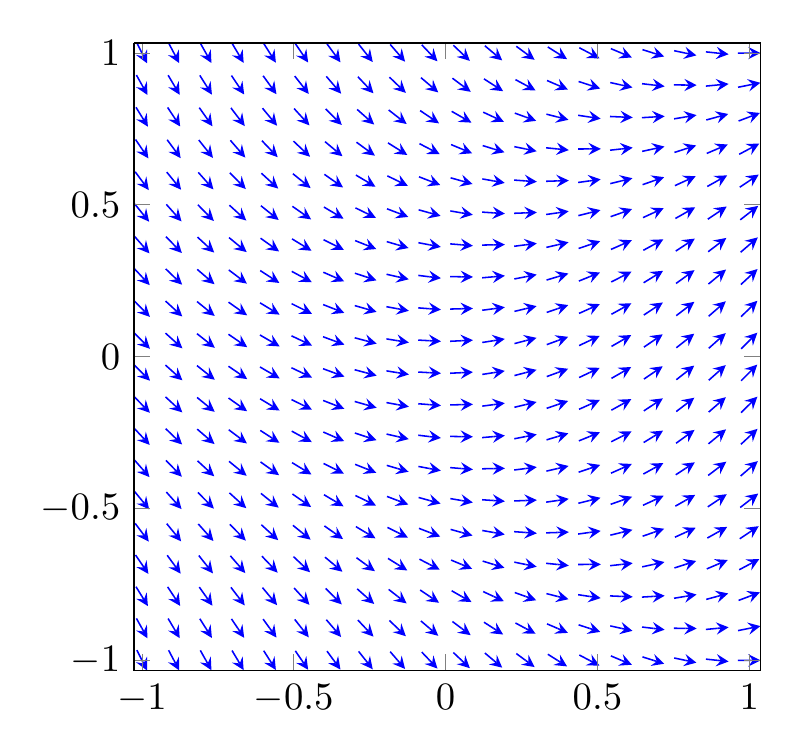
\begin{tikzpicture}[scale=1.4,
    declare function = {f(\x) = \x-\y*\y;} % Define which function we're using
    ]
    \begin{axis}[
        zmax = 1,
        zmin = 0,
        xtick = {-1,-0.5,...,1},
        axis equal image = true, % Unit vectors for both axes have the same length
        view = {0}{90}
        ]
        \addplot3[% Arrows' first-half
            blue,
            -stealth,
            domain  = -1:1,
            samples = 20,
            quiver  = {
                u=1/(2*sqrt(1^2 + f(x)^2)),
                v=f(x)/(2*sqrt(1^2 + f(x)^2)),
                scale arrows=0.075,
                },
        ] (x,y,0);
        \addplot3[% Arrow's second-half
            blue,
            domain  = -1:1,
            samples = 20,
            quiver  = {
                u=-1/(2*sqrt(1^2 + f(x)^2)),
                v=-f(x)/(2*sqrt(1^2 + f(x)^2)),
                scale arrows=0.075,
                },
        ] (x,y,0);
    \end{axis}
\end{tikzpicture}
\caption{A direction field}
\end{figure}

 Let $f(x,y)=x-y^2$, $y_0=1$ and $x_i=0+i\Delta x$ for $i=1,2,...,10$. Then\\

 $y_1=y_0+f(x_0,y_0)\Delta x=1+[0-1^2](0.1)=0.9$,\\

 $y_2=y_1+f(x_1,y_1)\Delta x=0.9+[0.1-(0.9)^2](0.1)=0.829$,\\

 $y_3=y_2+f(x_2,y_2)\Delta x=0.829+[0.2-(0.829)^2](0.1)=0.7802759$, \\

 $y_4=y_3+f(x_3,y_3)\Delta x=0.7802759+[0.3-(0.7802759)^2](0.1)=0.74939285198$,\\

 $y_5=y_4+f(x_4,y_4)\Delta x=0.74939285198+[0.4-(0.74939285198)^2](0.1)=0.73323388732$, \\

 $y_6=y_5+f(x_5,y_5)\Delta x=0.73323388732+[0.5-(0.73323388732)^2](0.1)=0.72947069396$, \\

 $y_7=y_6+f(x_6,y_6)\Delta x=0.72947069396+[0.6-(0.72947069396)^2](0.1)=0.73625794462$, \\

 $y_8=y_7+f(x_7,y_7)\Delta x=0.73625794462+[0.7-(0.73625794462)^2](0.1)=0.75205036851$, \\

 $y_9=y_8+f(x_8,y_8)\Delta x=0.75205036851+[0.8-(0.75205036851)^2](0.1)=0.77549239283$, \\

 $y_{10}=y_9+f(x_9,y_9)\Delta x=0.77549239283+[0.9-(0.77549239283)^2](0.1)=0.80535354769$. \\

 So $y(1)\approx y_{10}\approx 0.81$.



\end{document}